\documentclass{article}
\usepackage[utf8]{inputenc}
\usepackage{amsmath}
\usepackage{amssymb}
\usepackage{graphicx}
\usepackage{xcolor}
\usepackage{centernot}

\begin{document}
\section*{Fitting of (relative) Point Locations from Distances}

The numbers $x_{1}, \dots, x_{n} \in \mathbb{R}$ describe the location of $n$ points lying on a line that is identified with the real axis $\mathbb{R}$. We now receive $m := \binom{n}{2} = \frac{1}{2}n\left(n-1\right)$ values for (signed) distances
\begin{equation*}
    d_{i,j} := x_{j} - x_{j} \in \mathbb{R}
\end{equation*}
for $1 \leq i < j \leq n$, from which then determine the $x_{1}, x_{2}, \dots, x_{n}$ up to a shift. Setting $x_{n} := 0$ does fix the shift. This leads to the following overdetermined linear system of equations
\begin{equation*}
    \begin{cases}
    x_{j}-x_{i} = d_{i,j}\,,\quad &1 \leq i < j \leq n - 1\,,\\
    \phantom{x_{j}}-x_{i} = d_{i,n}\,,&i\in\left\{1, \dots, n-1\right\}
    \end{cases}
\end{equation*}
The unknowns are given by $\mathbf{x} = \left[x_{1}, \dots, x_{n-1}\right]^{\mathsf{T}} \in \mathbb{R}^{n-1}$. We can then recast this as an $m \times \left(n-1\right)$ linear system of equations $\mathbf{A}\mathbf{x} = \mathbf{b}$ where $\mathbf{b} \in \mathbb{R}^{m}$ contains each of the distances $d_{i,j}$, $1 \leq i < j \leq n$ exactly once. Let us first look a bit more at the mentioned recast linear system of equations $\mathbf{A}\mathbf{x} = \mathbf{b}$. We can see that we get the system (one of many possible systems)
\begin{equation*}
    \begin{bmatrix}
    \color{red}-1\color{black} & \color{blue}1\color{black} & 0 & 0 & \dots & 0 & 0\\
    \color{red}-1\color{black} & 0 & \color{blue}1\color{black} & 0 & \dots & 0 & 0\\
    \color{red}-1\color{black} & 0 & 0 & \color{blue}1\color{black} & \dots & 0 & 0\\
    \vdots & \vdots & \vdots & \vdots & & \vdots & \vdots \\
    \color{red}-1\color{black} & 0 & 0 & 0 & \dots & 0 & \color{blue}1\color{black}\\
    \color{teal}-1\color{black} & 0 & 0 & 0 & \dots & 0 & \color{black}0\color{black}\\
    0 & \color{red}-1\color{black} & \color{blue} 1\color{black} & 0 & \dots & 0 & 0 \\
    0 & \color{red}-1\color{black} & 0 & \color{blue}1\color{black} & \dots & 0 & 0\\
    \vdots & \vdots & \vdots & \vdots & & \vdots & \vdots\\
    0 & \color{red}-1\color{black} & 0 & 0 & \dots & 0 & \color{blue}1\color{black}\\
    0 & \color{teal}-1\color{black} & 0 & 0 & \dots & 0 & \color{black}0\color{black}\\
    \vdots & \vdots & \vdots & \vdots & & \vdots& \vdots \\
    \vdots & \vdots & \vdots & \vdots & & \vdots& \vdots \\
    0 & 0 & 0 & 0 & \dots & \color{red}-1\color{black} & \color{blue}1\color{black}\\
    0 & 0 & 0 & 0 & \dots  &\color{teal}-1\color{black} & 0 \\
    0 & 0 & 0 & 0 & \dots & 0 &\color{teal}-1\color{black} \\
    \end{bmatrix}
    \begin{bmatrix}
        x_{1} \\ x_{2} \\ x_{3} \\ x_{4} \\ \dots \\ x_{n-2} \\ x_{n-1}
    \end{bmatrix} = 
    \begin{bmatrix}
        d_{\color{red}1\color{black},\color{blue}1\color{black}} \\
        d_{\color{red}1\color{black},\color{blue}2\color{black}} \\
        d_{\color{red}1\color{black},\color{blue}3\color{black}} \\
        \vdots \\
        d_{\color{red}1\color{black},\color{blue}n-1\color{black}} \\
        d_{\color{teal}1\color{black},\color{teal}n\color{black}} \\
        d_{\color{red}2\color{black},\color{blue}3\color{black}} \\
        d_{\color{red}2\color{black},\color{blue}4\color{black}} \\
        \vdots  \\
        d_{\color{red}2\color{black},\color{blue}n-1\color{black}} \\
        d_{\color{teal}2\color{black},\color{teal}n\color{black}} \\
        \vdots  \\
         \vdots \\
         d_{\color{red}n-2\color{black},\color{blue}n-1\color{black}} \\
         d_{\color{teal}n-2\color{black},\color{teal}n\color{black}} \\
         d_{\color{teal}n-1\color{black},\color{teal}n\color{black}}
    \end{bmatrix}
\end{equation*}
\subsection*{3-10.a}
We are tasked with determining how many real numbers and integers have to be stored at least in order to represent the matrix $\mathbf{A}$ int COO/triplet format and CRS format.

\paragraph{COO / triplet format:} In the triplet format we store at least two triplets per row as we have exactly two non-zero entries per row of the matrix, besides for for $\left(n-1\right)$ entries that correspond to $d_{i,n}$ they will only contain one entry. We can hence compute the amount of triplets by subtracting these from the total produced by $2 \cdot m$
\begin{equation*}
    \text{\# triplets } \geq 2 \cdot m - \left(n-1\right) = 2 \cdot \frac{1}{2}n\left(n-1\right) - \left(n-1\right) = n^{2} - n - n + 1 = \left(n-1\right)^{2}
\end{equation*}
The triplets contain two entries which give us the row and the column which both are integers and one entry that is a real number giving us the contents of said row (or at least a part of it, because multiple triplets with the same row, columns can exist). This thus gives us at least $2\left(n-1\right)^{2}$ integers and $\left(n-1\right)$ real numbers.

\paragraph{Compressed row-storage (CRS) format:} The definition of the three arrays used in the CRS format is given by

\begin{figure}[!hbt]
    \centering
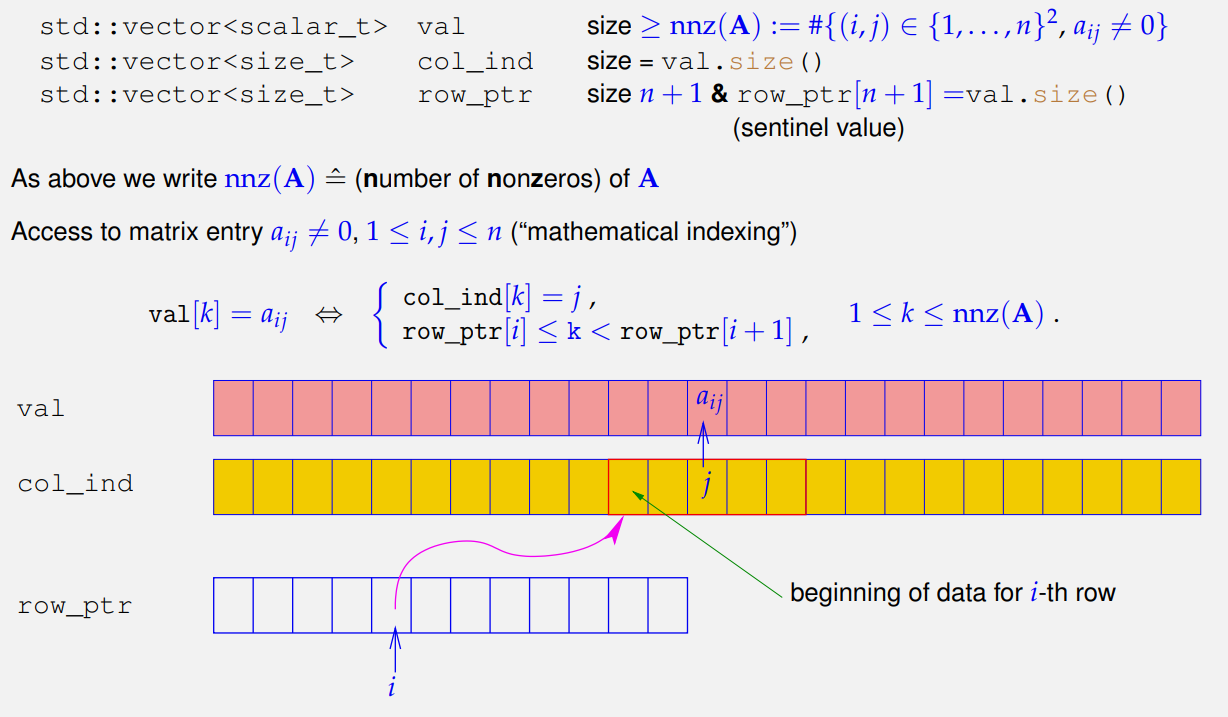
\includegraphics[width=1.0\linewidth]{CRSFormatDef.png}
\end{figure}
\noindent From this we can see that \verb|row_ptr| has $m+1$ entries as we have an additional entry at the end which is used to make it easier to iterate over the structure. We can then also see that both \verb|col_ind| and \verb|val| contain at least one entry per entry in the given matrix, which gives us at least $\left(n-1\right)^{2}$ entries. Because \verb|row_ptr| and \verb|col_ind| both contain integers whereas \verb|val| contains real numbers. Which thus gives us at least 
\begin{equation*}
  \left(n-1\right)^{2} + \frac{1}{2}n\left(n-1\right)^{2}  + 1= n^{2} - 2n + 1 + \frac{1}{2}n^{2} - \frac{1}{2} +1  = \left(\frac{3}{2}n - 1\right)\left(n-1\right)
\end{equation*}
integers and $\left(n-1\right)^{2}$ real numbers.

\pagebreak

\subsection*{3-10.b}
We are tasked with implementing a method \verb|initA| that initializes the matrix $\mathbf{A}$ according to the above structure. For this we must first consider chapter 2.7.2 on sparse matrices in Eigen. It tells us that by including \verb|<Eigen/Sparse>| we can use the type \verb|Eigen::SparseMatrix<double>|. It also tells us that we should initialize the sparse matrix type using first a vector of triplets and then use this vector in combination to \verb|setFromTriplets| to construct the sparse matrix.  

\begin{figure}[!hbt]
    \centering
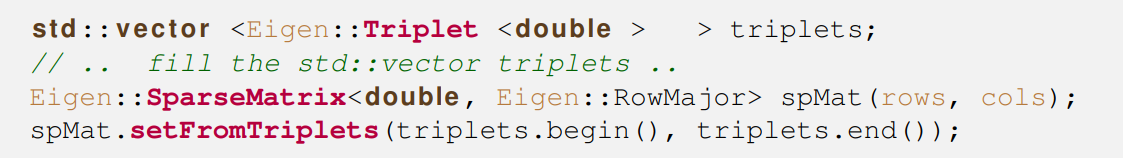
\includegraphics[width=1.0\linewidth]{SparseMatrixFromTriplets.png}
\end{figure}

\noindent Following this structure gives us the following code (keep in mind that the system is a $m \times \left(n - 1\right)$ system.)
\begin{figure}[!hbt]
    \centering
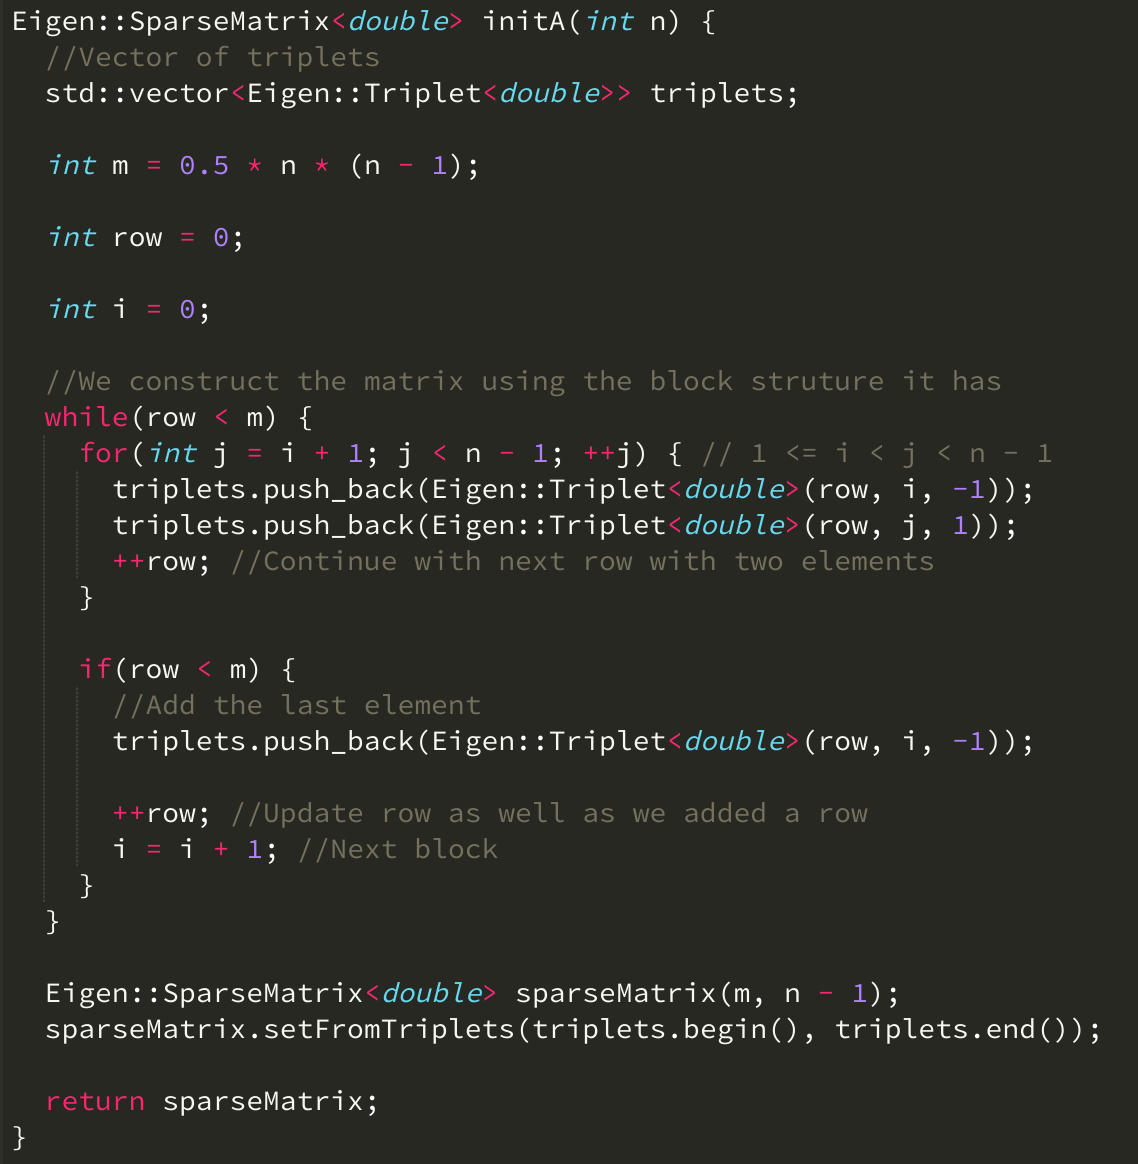
\includegraphics[width=0.9\linewidth]{3-10.b.png}
\end{figure}

\pagebreak

\subsection*{3-10.c}
We now are interested in implementing a solver for the given system of equations. To this extent we will use extended normal equations and the use the block structure of the given matrix to achieve this. For an overdetermined linear system $\mathbf{M}\mathbf{x} = \mathbf{c}$, $\mathbf{M} \in \mathbb{R}^{m,l}$, $\mathbf{c} \in \mathbb{R}^{m}$, $m \geq l$ we get 
\begin{equation*}
    \begin{bmatrix}
        -\mathbf{I} & \mathbf{M} \\
        \mathbf{M}^{\mathsf{T}} & \mathbf{O}
    \end{bmatrix}
    \begin{bmatrix}
        \mathbf{r} \\
        \mathbf{x}
    \end{bmatrix}
    =
    \begin{bmatrix}
        \mathbf{c} \\
        \mathbf{0}
    \end{bmatrix}
\end{equation*}
We can use the sparse direct solver provided by Eigen to solve the extended normal equations for the position fitting problem discussed in this exercise and returns its least-squares solution $\mathbf{x}\in \mathbb{R}^{n-1}$. The argument \verb|D| passes an $\left(n \times n\right)$ matrix $\mathbf{D}$ whose strict upper triangular part contains the distances 
\begin{equation*}
    \mathbf{D}_{i,j} = d_{i, j}\,,\quad 1 \leq i < j \leq n
\end{equation*}
Our goal is thus to solve for the found matrix $\mathbf{A}$ of the given overdetermined linear systems of equations to find the least-squares solution of
\begin{equation*}
\underbrace{
    \begin{bmatrix}
        -\mathbf{I} &  \mathbf{A} \\
        \mathbf{A}^{\mathsf{T}} & \mathbf{O}
    \end{bmatrix}}_{=\mathbf{A}_{\text{ext}}}
    \begin{bmatrix}
        \mathbf{r} \\
        \mathbf{x}
    \end{bmatrix}
    = 
    \begin{bmatrix}
        \mathbf{c} \\
        \mathbf{0}
    \end{bmatrix}
\end{equation*}
We again use triplets to build the block matrix $\mathbf{A}_{\text{ext}}$. We can reuse our nested loops from 3-10.b to do so. Sadly we cannot use \verb|<<| or block operations on sparse matrices, hence we have to shift the triplets row / column values. For $\mathbf{A}^{\mathsf{T}}$ we do switch row and columns and also shift the triplets. For the $\mathbf{O}$ block we do not have to do anything. We have $\mathbf{A} \in \mathbb{R}^{m,l}$ and thus $\mathbf{A}^{\mathsf{T}} \in \mathbb{R}^{l,m}$ and as a consequence $\mathbf{I} \in \mathbb{R}^{m,m}$. This then produces a $\left(m + n - 1\right) \times \left(m+n-1\right)$ block matrix. For debugging purposes triplets can be output by using \verb|triplet.row()|, \verb|triplet.col()| and \verb|triplet.value()| for a given triplet \verb|triplet|. We first give the code for adding the Identity block and construct the matrix. 

\begin{figure}[!hbt]
    \centering
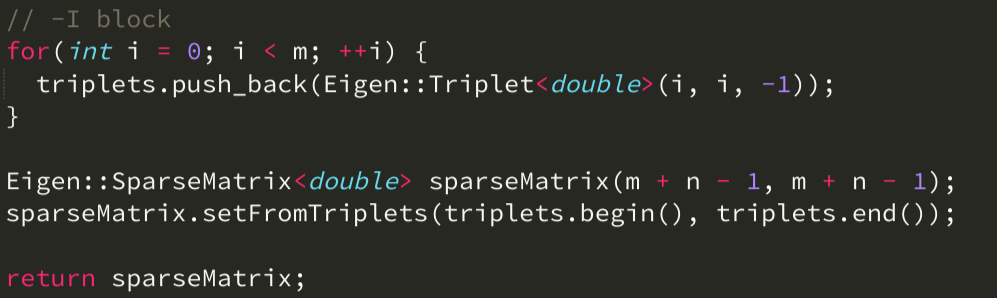
\includegraphics[width=1.0\linewidth]{3-10.c_2.png}
\end{figure}

\pagebreak

\noindent Here is the code for the modified while loop.

\begin{figure}[!hbt]
    \centering
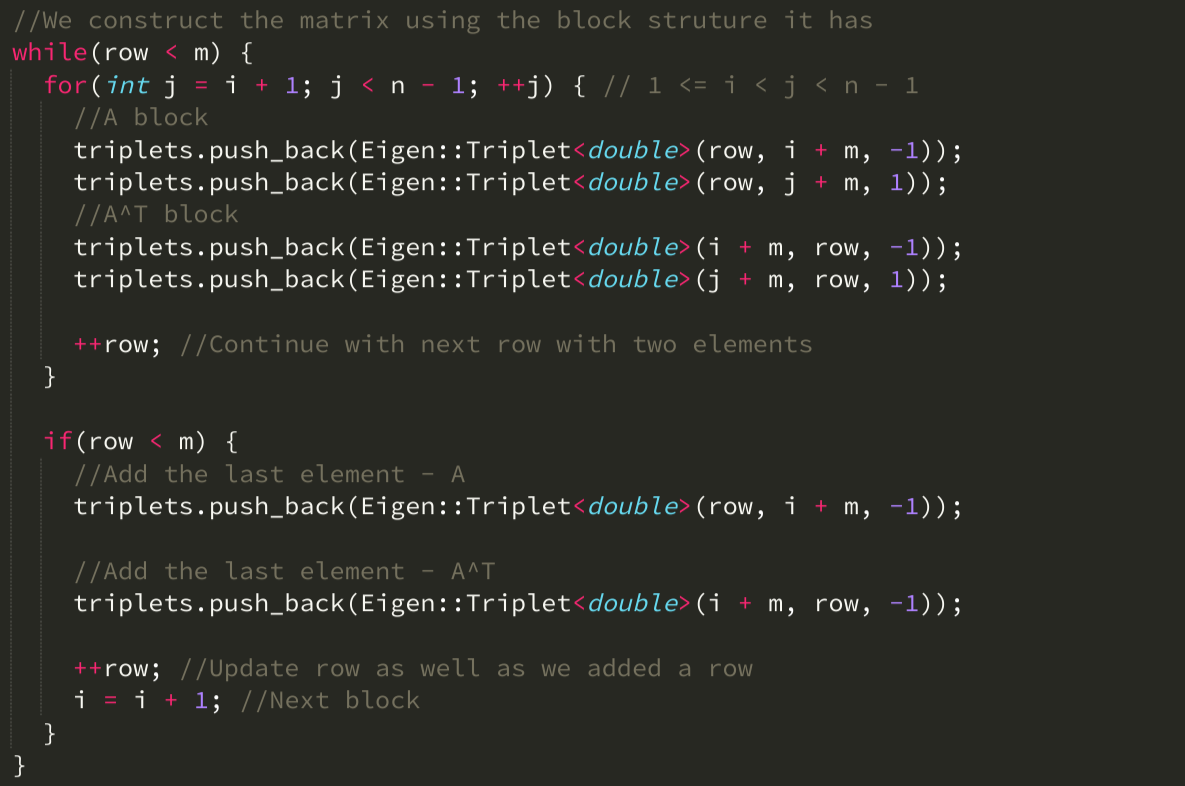
\includegraphics[width=1.0\linewidth]{3-10.c_1.png}
\end{figure}


\noindent One can use \verb|<<| to output the sparse matrix non-zero entries, the \verb|row_ptr| entries (I believe that Eigen is column-major by default, so more like the \verb|col_ptr| entries) called outer pointers and the matrix itself. This matrix is structured very poorly and it is thus difficult to see if the matrix is correctly formatted. After writing a method by ourselves with a bit of spacing we can see the structure.

\begin{figure}[!hbt]
    \centering
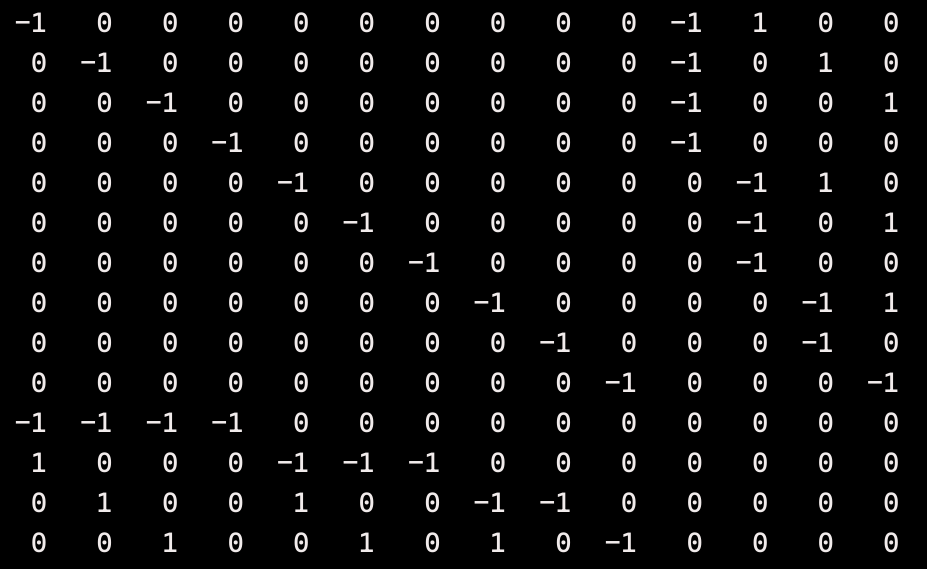
\includegraphics[width=0.7\linewidth]{SparseMatrixStructure.png}
\end{figure}

\noindent Now we want to solve the extended normal equations. We remember from section 3.2.0.7 that the extended normal equations are used because they preserve the sparsity of the matrix $\mathbf{A}$ when computing $\mathbf{A}^{\mathsf{T}}\mathbf{A}$. This is because we have 

\begin{equation*}
    \mathbf{A} \text{ sparse } \centernot\implies \mathbf{A}^{\mathsf{T}}\mathbf{A} \text{ sparse}
\end{equation*}

\noindent This can lead to memory overflow when we compute $\mathbf{A}^{\mathsf{T}}\mathbf{A}$ and makes it impossible to use efficient sparse direct elimination techniques. Preserving the structure we can thus use \verb|Eigen::SparseLU| to solve the normal equations. The entries of the vector $\left[\mathbf{c}, \mathbf{0}\right]^{\mathsf{T}}$ are given by $d_{i,j}$, which are entries of the matrix given as input. We will use the same navigation pattern as when constructing $\mathbf{A}$ to move through the matrix $\mathbf{D}$ to extract these entries in the right order. This produces the following method to construct the right-hand side vector of the block system.

\begin{figure}[!hbt]
    \centering
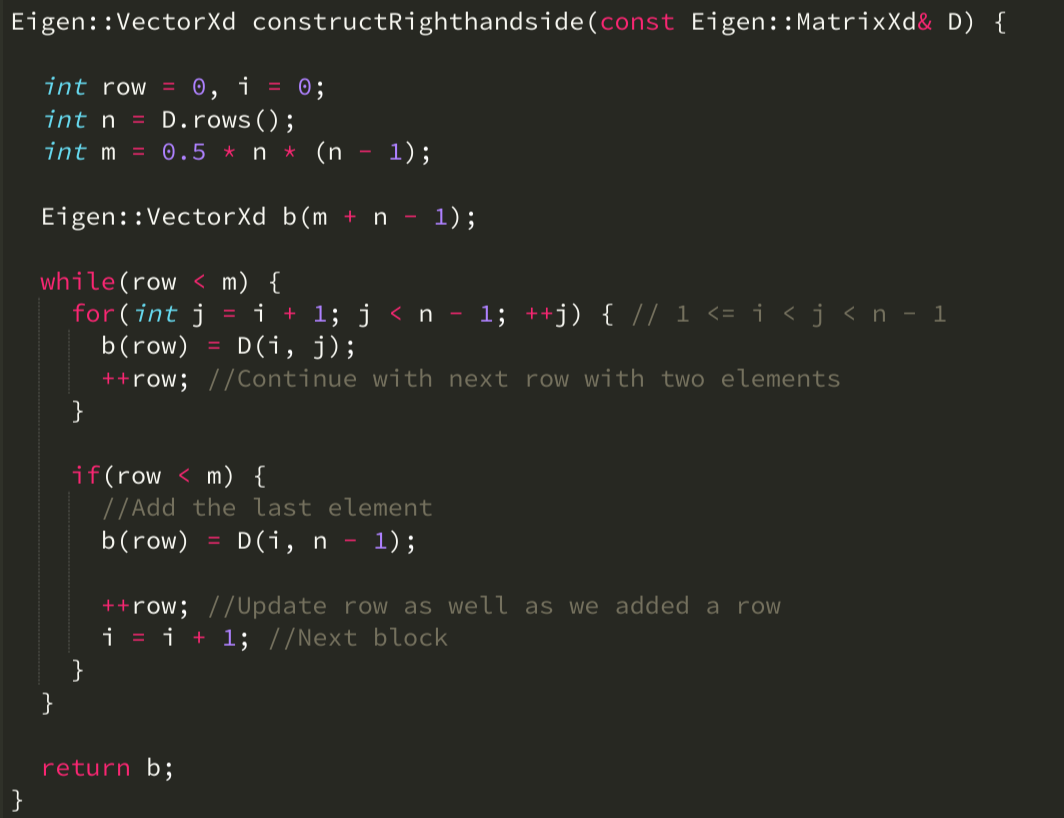
\includegraphics[width=0.7\linewidth]{3-10.c_3.png}
\end{figure}

\noindent Having constructed the block system, we can now solve the extended normal equations, just as we would solve the conventional normal equations. We have 
\begin{equation*}
    \mathbf{A}^{\mathsf{T}}\mathbf{A}\mathbf{x} = \mathbf{A}^{\mathsf{T}}\mathbf{b} \Longleftrightarrow  
    \begin{bmatrix}
        -\mathbf{I} &  \mathbf{A} \\
        \mathbf{A}^{\mathsf{T}} & \mathbf{O}
    \end{bmatrix}
    \begin{bmatrix}
        \mathbf{r} \\
        \mathbf{x}
    \end{bmatrix}
    = 
    \begin{bmatrix}
        \mathbf{c} \\
        \mathbf{0}
    \end{bmatrix}
\end{equation*}

\noindent To aid us in implementing solving the extended normal equations we use the following code segment from the lecture document (2.7.3).

\begin{figure}[!hbt]
    \centering
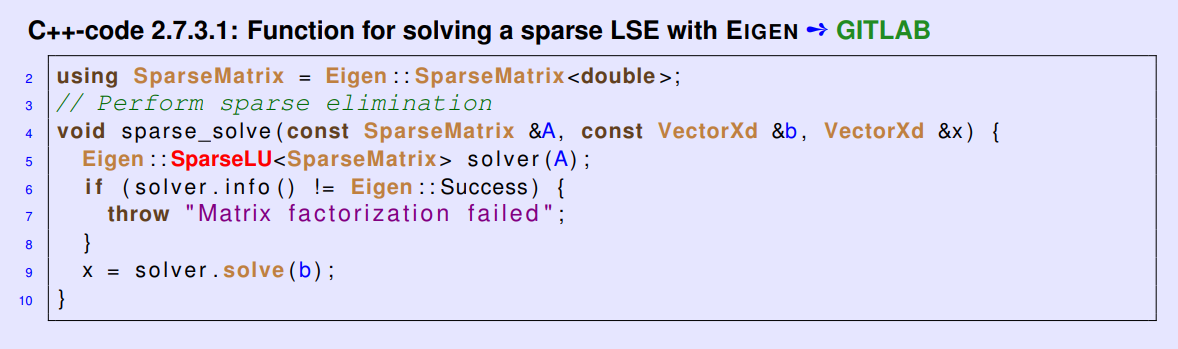
\includegraphics[width=1.0\linewidth]{LUSolverFunction.png}
\end{figure}

\noindent We do not compute any products that destroy the sparsity of the system anymore, hence we can use sparse solvers. The vector $\mathbf{r}$ is the residual, i.e. $\mathbf{r} = \mathbf{A}\mathbf{x} - \mathbf{b}$. We are here only interested in $\mathbf{x}$ hence we will only return these elements. This produces the following code which calls our helper functions.

\begin{figure}[!hbt]
    \centering
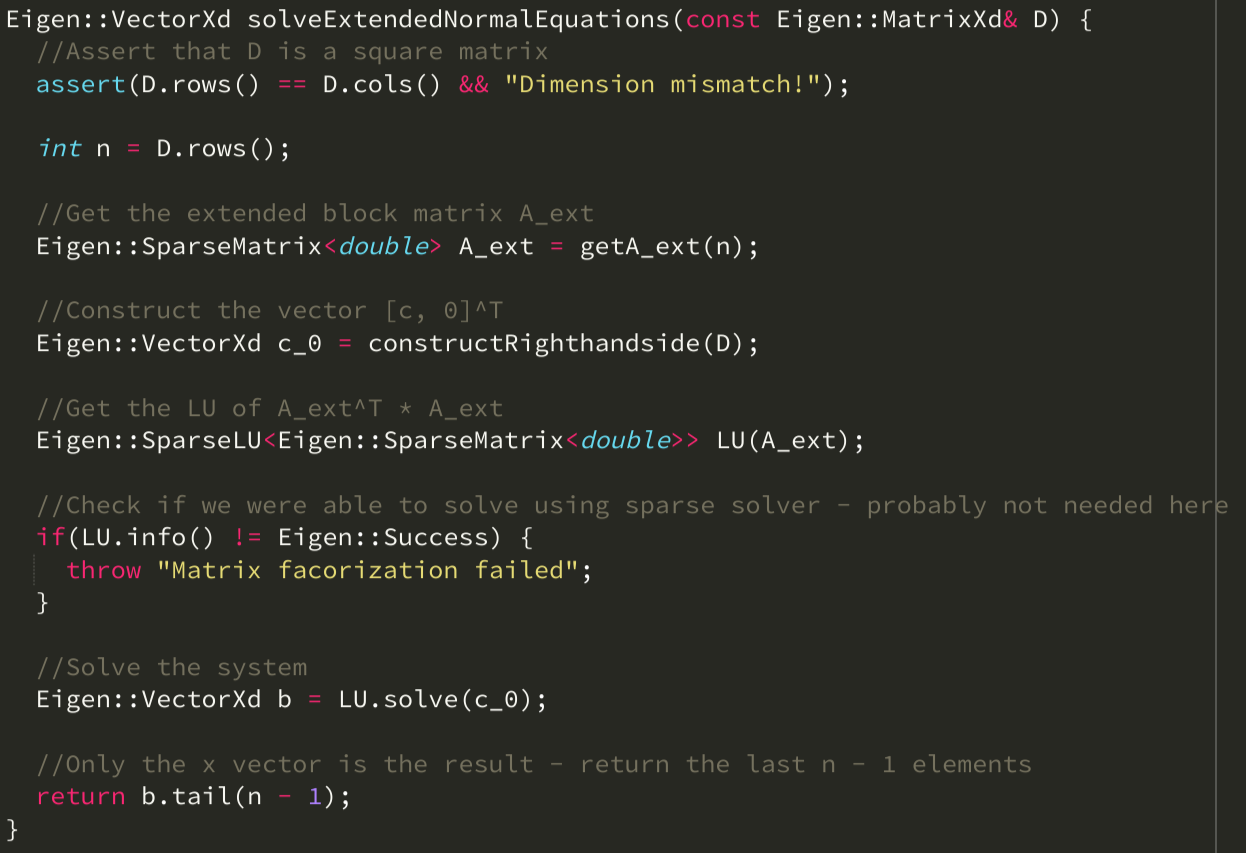
\includegraphics[width=1.0\linewidth]{3-10.c_4.png}
\end{figure}

\subsection*{3-10.d}
The coefficient matrix $\mathbf{M} \in \mathbb{R}^{n-1, n-1}$ of the normal equations associated with the overdetermined linear system 

\begin{equation*}
    \begin{cases}
    x_{j}-x_{i} = d_{i,j}\,,\quad &1 \leq i < j \leq n - 1\,,\\
    \phantom{x_{j}}-x_{i} = d_{i,n}\,,&i\in\left\{1, \dots, n-1\right\}
    \end{cases}
\end{equation*}
is of the form 
\begin{equation*}
    \mathbf{M} = \mathbf{D} - \mathbf{z}\mathbf{z}^{\mathsf{T}} \text{ with } \quad \begin{matrix} \hspace{9px}\text{a diagonal matrix } \mathbf{D} \in \mathbb{R}^{n-1,n-1} \\
    \text{and a column vector } \mathbf{z} \in \mathbb{R}^{n-1}
    \end{matrix}
\end{equation*}
We are tasked with computing $\mathbf{D}$ and $\mathbf{z}$ and then find a simple expression for the inverse $\mathbf{M}^{-1}$. Let us first find a suitable vector $\mathbf{z}$. The matrix $\mathbf{D}$ is not the same as above, we have
\begin{equation*}
    \mathbf{D} = 
    \begin{bmatrix}
        d_{1,1} & 0 & \dots & 0\\
        0  & d_{2,2} & \dots & 0 \\
        \vdots & & \ddots  & \vdots \\
        0  & \dots& 0 & d_{n-1,n-1} 
    \end{bmatrix}
\end{equation*}

\pagebreak

\noindent We now look at the structure of $\mathbf{M}$, this is explained less than optimal because it took me a long time to realize that $\mathbf{M} = \mathbf{A}^{\mathsf{T}}\mathbf{A}$ which makes sense considering that $\mathbf{M} \in \mathbb{R}^{n-1, n-1}$, but before we had $\mathbf{M} = \mathbf{A}$. This aside we have for $\mathbf{A}$

\begin{equation*}
\mathbf{A} = 
\begin{bmatrix}
    -1& 1 & 0 & 0 & \dots & 0 & 0\\
    -1 & 0 & 1 & 0 & \dots & 0 & 0\\
    -1 & 0 & 0 & 1 & \dots & 0 & 0\\
    \vdots & \vdots & \vdots & \vdots & & \vdots & \vdots \\
    -1 & 0 & 0 & 0 & \dots & 0 & 1\\
    -1 & 0 & 0 & 0 & \dots & 0 & 0\\
    0 & -1 &  1 & 0 & \dots & 0 & 0 \\
    0 & -1 & 0 & 1 & \dots & 0 & 0\\
    \vdots & \vdots & \vdots & \vdots & & \vdots & \vdots\\
    0 & -1 & 0 & 0 & \dots & 0 & 1\\
    0 &-1 & 0 & 0 & \dots & 0 & 0\\
    \vdots & \vdots & \vdots & \vdots & & \vdots& \vdots \\
    \vdots & \vdots & \vdots & \vdots & & \vdots& \vdots \\
    0 & 0 & 0 & 0 & \dots & -1 & 1\\
    0 & 0 & 0 & 0 & \dots  &-1& 0 \\
    0 & 0 & 0 & 0 & \dots & 0 &-1 \\
    \end{bmatrix}
\end{equation*}
Understanding what happens when computing $\mathbf{M} = \mathbf{A}^{\mathsf{T}}$ from this will be challenging hence let us consider a small example.
\begin{align*}
    \mathbf{M} &= 
    \underbrace{\begin{bmatrix}
       -1 & - 1 & -1 & -1  & \phantom{-}0 & \phantom{-}0 & \phantom{-}0 & \phantom{-}0 & \phantom{-}0 & \phantom{-}0 \\
        \phantom{-}1 & \phantom{-}0 & \phantom{-}0 & \phantom{-}0 & -1 & - 1 & -1 & \phantom{-}0 & \phantom{-}0 & \phantom{-}0 \\
        \phantom{-}0 & \phantom{-}1 & \phantom{-}0 & \phantom{-}0  & \phantom{-}1 & \phantom{-}0 & \phantom{-}0 & -1 & -1 & \phantom{-}0 \\
        \phantom{-}0 & \phantom{-}0 & \phantom{-}1 & \phantom{-}0  & \phantom{-}0 & \phantom{-}1 & \phantom{-}0 & \phantom{-}1 & \phantom{-}0 & -1      
    \end{bmatrix}}_{= \mathbf{A}^{\mathsf{T}}}
    \underbrace{\begin{bmatrix}
    -1& \phantom{-}1 & \phantom{-}0  & \phantom{-}0 \\
    -1 & \phantom{-}0 & \phantom{-}1  & \phantom{-}0 \\
    -1 & \phantom{-}0 & \phantom{-}0 & \phantom{-}1 \\
    -1 & \phantom{-}0 & \phantom{-}0 & \phantom{-}0 \\
    \phantom{-}0 & -1 & \phantom{-}1 & \phantom{-}0 \\
    \phantom{-}0 & -1 & \phantom{-}0 & \phantom{-}1 \\
    \phantom{-}0 & -1 & \phantom{-}0 & \phantom{-}0 \\
    \phantom{-}0 & \phantom{-}0 & -1 & \phantom{-}1 \\
    \phantom{-}0 & \phantom{-}0 & -1 & \phantom{-}0 \\
    \phantom{-}0 & \phantom{-}0 & \phantom{-}0 & -1 \\
    \end{bmatrix}}_{= \mathbf{A}} \\[2mm]
    &= \begin{bmatrix}
        \mathbf{A}^{\mathsf{T}}_{1:1,1:10} \\
        \mathbf{A}^{\mathsf{T}}_{2:2,1:10} \\
        \mathbf{A}^{\mathsf{T}}_{3:3,1:10} \\
        \mathbf{A}^{\mathsf{T}}_{4:4,1:10}
    \end{bmatrix}
    \begin{bmatrix}
        \mathbf{A}_{1:10, 1:1} &
        \mathbf{A}_{1:10, 2:2} &
        \mathbf{A}_{1:10, 3:3} &
        \mathbf{A}_{1:10, 4:4} &
        \end{bmatrix} 
\end{align*}
The notation $\mathbf{A}^{\mathsf{T}}_{i:i,1:m}$ means the $i$-th row (has length $m$) of $\mathbf{A}^{\mathsf{T}}$ and the notation  $\mathbf{A}_{1:m, i:i}$ means the $i$-th row of $\mathbf{A}$ (has length $m$).

\pagebreak

\noindent We proceed from here 
\begin{align*}
\dots &=
     \begin{bmatrix}
        \mathbf{A}^{\mathsf{T}}_{1:1,1:10} \\
        \mathbf{A}^{\mathsf{T}}_{2:2,1:10} \\
        \mathbf{A}^{\mathsf{T}}_{3:3,1:10} \\
        \mathbf{A}^{\mathsf{T}}_{4:4,1:10}
    \end{bmatrix}
    \begin{bmatrix}
        \mathbf{A}_{1:10, 1:1} &
        \mathbf{A}_{1:10, 2:2} &
        \mathbf{A}_{1:10, 3:3} &
        \mathbf{A}_{1:10, 4:4} &
        \end{bmatrix}  \\[2mm]
        &= \begin{bmatrix}
            \mathbf{A}^{\mathsf{T}}_{1:1,1:10}\mathbf{A}_{1:10, 1:1} & 
            \mathbf{A}^{\mathsf{T}}_{1:1,1:10}\mathbf{A}_{1:10, 2:2} & 
            \mathbf{A}^{\mathsf{T}}_{1:1,1:10}\mathbf{A}_{1:10, 3:3} & 
            \mathbf{A}^{\mathsf{T}}_{1:1,1:10}\mathbf{A}_{1:10, 4:4} &  \\
            \mathbf{A}^{\mathsf{T}}_{2:2,1:10}\mathbf{A}_{1:10, 1:1} & 
            \mathbf{A}^{\mathsf{T}}_{2:2,1:10}\mathbf{A}_{1:10, 2:2} & 
            \mathbf{A}^{\mathsf{T}}_{2:2,1:10}\mathbf{A}_{1:10, 3:3} & 
            \mathbf{A}^{\mathsf{T}}_{2:2,1:10}\mathbf{A}_{1:10, 4:4} &  \\
            \mathbf{A}^{\mathsf{T}}_{3:3,1:10}\mathbf{A}_{1:10, 1:1} & 
            \mathbf{A}^{\mathsf{T}}_{3:3,1:10}\mathbf{A}_{1:10, 2:2} & 
            \mathbf{A}^{\mathsf{T}}_{3:3,1:10}\mathbf{A}_{1:10, 3:3} & 
            \mathbf{A}^{\mathsf{T}}_{3:3,1:10}\mathbf{A}_{1:10, 4:4} &  \\
            \mathbf{A}^{\mathsf{T}}_{4:4,1:10}\mathbf{A}_{1:10, 1:1} & 
            \mathbf{A}^{\mathsf{T}}_{4:4,1:10}\mathbf{A}_{1:10, 2:2} & 
            \mathbf{A}^{\mathsf{T}}_{4:4,1:10}\mathbf{A}_{1:10, 3:3} & 
            \mathbf{A}^{\mathsf{T}}_{4:4,1:10}\mathbf{A}_{1:10, 4:4} & 
        \end{bmatrix}
\end{align*}
I am aware that this helps little with seeing the actual structure, however it shows that each entry is an inner product, which is crucial. Our example then gives us
\begin{align*}
     \mathbf{M} &= 
    \begin{bmatrix}
       -1 & - 1 & -1 & -1  & \phantom{-}0 & \phantom{-}0 & \phantom{-}0 & \phantom{-}0 & \phantom{-}0 & \phantom{-}0 \\
        \phantom{-}1 & \phantom{-}0 & \phantom{-}0 & \phantom{-}0 & -1 & - 1 & -1 & \phantom{-}0 & \phantom{-}0 & \phantom{-}0 \\
        \phantom{-}0 & \phantom{-}1 & \phantom{-}0 & \phantom{-}0  & \phantom{-}1 & \phantom{-}0 & \phantom{-}0 & -1 & -1 & \phantom{-}0 \\
        \phantom{-}0 & \phantom{-}0 & \phantom{-}1 & \phantom{-}0  & \phantom{-}0 & \phantom{-}1 & \phantom{-}0 & \phantom{-}1 & \phantom{-}0 & -1      
    \end{bmatrix}
    \begin{bmatrix}
    -1& \phantom{-}1 & \phantom{-}0  & \phantom{-}0 \\
    -1 & \phantom{-}0 & \phantom{-}1  & \phantom{-}0 \\
    -1 & \phantom{-}0 & \phantom{-}0 & \phantom{-}1 \\
    -1 & \phantom{-}0 & \phantom{-}0 & \phantom{-}0 \\
    \phantom{-}0 & -1 & \phantom{-}1 & \phantom{-}0 \\
    \phantom{-}0 & -1 & \phantom{-}0 & \phantom{-}1 \\
    \phantom{-}0 & -1 & \phantom{-}0 & \phantom{-}0 \\
    \phantom{-}0 & \phantom{-}0 & -1 & \phantom{-}1 \\
    \phantom{-}0 & \phantom{-}0 & -1 & \phantom{-}0 \\
    \phantom{-}0 & \phantom{-}0 & \phantom{-}0 & -1 \\
    \end{bmatrix} \\[1mm]
    &= \begin{bmatrix}
        4 & -1 & -1 & -1 \\
        -1 & 4 & -1 & -1 \\
        -1 & -1 & 4 & -1 \\
        -1 & -1 & -1 & 4
    \end{bmatrix} =
    \begin{bmatrix}
        n - 1& -1 & -1 & -1 \\
        -1 & n - 1 & -1 & -1 \\
        -1 & -1 & n -1& -1 \\
        -1 & -1 & -1 & n-1
    \end{bmatrix}
\end{align*}
It makes sense that we get $n-1$ (we get $k-1$ unknowns for $n = k$, here with $n = 5$)on the diagonal as we have exactly $n$ non-zero entries per row / column of $\mathbf{A}$ and they all are either $1$ or $-1$ and because in the diagonal case we will take the inner product of the same vector we hence must get $n$. We hence see that we get 
\begin{align*}
    \begin{bmatrix}
        n-1 & -1 & \dots & -1 \\
        -1 & n-1 & \dots & -1 \\
        \vdots & \vdots & \ddots & \vdots\\
        -1 & -1 & \dots & n-1
    \end{bmatrix} &= 
\underbrace{\begin{bmatrix}
        n & 0 & \dots & 0 \\
        0 & n & \dots & 0 \\
        \vdots & \vdots & \ddots & \vdots\\
        0 & 0 & \dots & n
    \end{bmatrix}}_{=\mathbf{D}} - 
    \underbrace{\begin{bmatrix}
        1 & 1 & \dots & 1 \\
        1 & 1 & \dots & 1 \\
        \vdots & \vdots & \ddots & \vdots\\
        1 & 1 & \dots & 1
    \end{bmatrix}}_{= \mathbf{z}\mathbf{z}^{\mathsf{T}}}
\end{align*}

\pagebreak

\noindent We hence get 
\begin{equation}
     \mathbf{M} = \mathbf{D} - \mathbf{z}\mathbf{z}^{\mathsf{T}}
\end{equation}
with $\mathbf{D} = \text{diag}\left(n, n, \dots, n\right)$ and $\mathbf{z} = \left[1, 1, \dots, 1\right]^{\mathsf{T}}$ with $\mathbf{D} \in \mathbb{R}^{n-1, n-1
}$ and $\mathbf{z} \in \mathbb{R}^{n-1}$. We can now see that the above equation implies a rank one modification, which then leads to the Sherman-Morrison-Woodbury formula.

\begin{figure}[!hbt]
    \centering
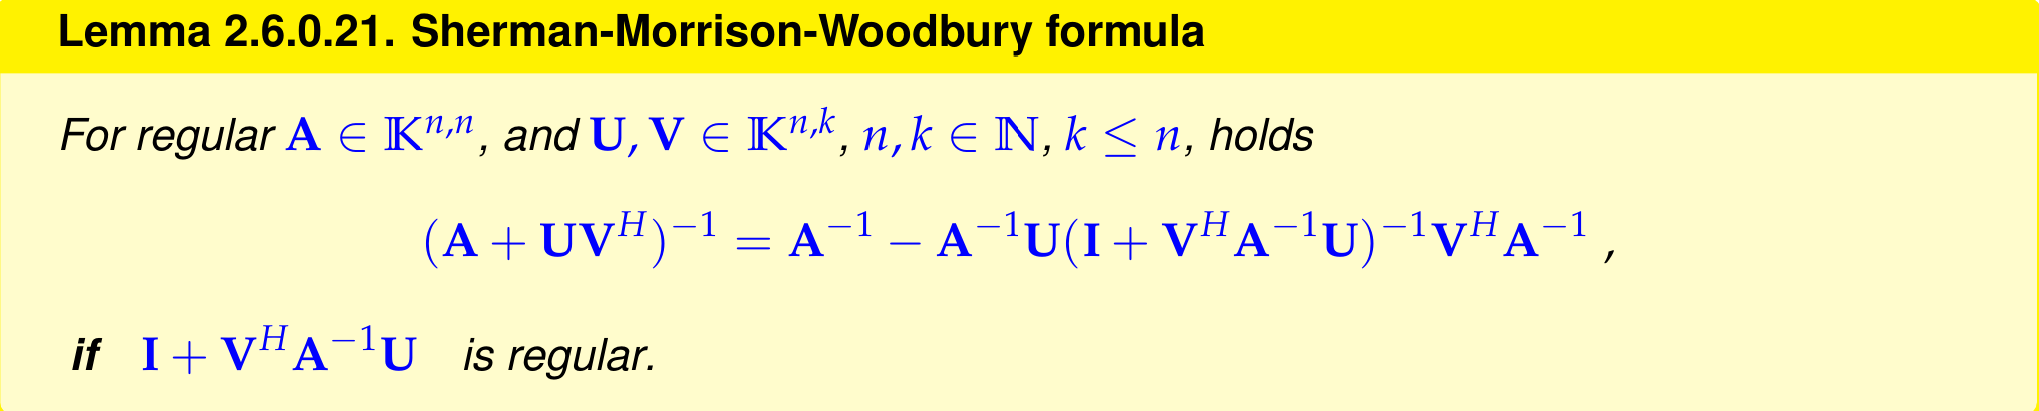
\includegraphics[width=1.0\linewidth]{ShermanMorrisonWoodbury.png}
\end{figure}

\noindent We see that our rank one modification is not exactly in this form, we would want to find to matrices $\mathbf{U}$ and $\mathbf{V}$ for which $\mathbf{M} = \mathbf{D} + \mathbf{U}\mathbf{V}^{\mathsf{T}}$. Choosing $k = 1$ in the definition also allows for $\mathbf{U}$ and $\mathbf{v}$ to be columns ($\in \mathbb{n-1}$). Hence we can see that
\begin{equation}
     \mathbf{M} = \mathbf{D} + \underbrace{\left(-\mathbf{z}\right)}_{=\mathbf{U}}\underbrace{\mathbf{z}^{\mathsf{T}}}_{=\mathbf{V}^{\mathsf{T}}}
\end{equation}
Defining $\mathbf{1} = \left[1, \dots, 1\right]^{\mathsf{T}} \in \mathbb{R}^{n-1}$ and $\mathbf{-1} = \left[-1, \dots, -1\right]^{\mathsf{T}} \in \mathbb{R}^{n-1}$ gives us 
\begin{equation*}
    \mathbf{M} = \mathbf{D} + \mathbf{-1}\mathbf{1}^{\mathsf{T}}
\end{equation*}
We hence get
\begin{align*}
    \mathbf{M}^{-1} = \left(\mathbf{D} + \mathbf{-1}\mathbf{1}^{\mathsf{T}}\right)^{-1} = \mathbf{D}^{-1} - \mathbf{D}^{-1}\mathbf{-1}\left(\mathbf{I} + \mathbf{1}^{\mathsf{T}}\mathbf{D}^{-1}\mathbf{-1}\right)^{-1}\mathbf{1}^{\mathsf{T}}\mathbf{D}^{-1}
\end{align*}
We know see that $\mathbf{D}= n\mathbf{I}$ and hence (because $\mathbf{D}$ is diagonal) we have as its inverse $\mathbf{D}^{-1} = \frac{1}{n}\mathbf{I}$. We also have $\mathbf{-1} = -1 \cdot \mathbf{I}$. The above can thus be written as 
\begin{align*}
     \left(\mathbf{D} + \mathbf{-1}\mathbf{1}^{\mathsf{T}}\right)^{-1} &= \mathbf{D}^{-1} - \mathbf{D}^{-1}\mathbf{-1}\left(\mathbf{I} + \mathbf{1}^{\mathsf{T}}\mathbf{D}^{-1}\mathbf{-1}\right)^{-1}\mathbf{1}^{\mathsf{T}}\mathbf{D}^{-1} \\
    &= \frac{1}{n}\mathbf{I} - \frac{1}{n}\mathbf{I}\mathbf{-1}\left(\mathbf{I} + \mathbf{1}^{\mathsf{T}}\frac{1}{n}\mathbf{I}\mathbf{-1}\right)^{-1}\mathbf{1}^{\mathsf{T}}\frac{1}{n}\mathbf{I} \quad \text{($\mathbf{D}^{-1} = \frac{1}{n}\mathbf{I}$)} \\
     &= \frac{1}{n}\mathbf{I} + \frac{1}{n^{2}}\mathbf{I}\mathbf{1}\left(\mathbf{I} -  \frac{1}{n}\mathbf{1}^{\mathsf{T}}\mathbf{I}\mathbf{1}\right)^{-1}\mathbf{1}^{\mathsf{T}}\mathbf{I} \quad \text{($\mathbf{-1} = -1\cdot \mathbf{1}$, $\frac{1}{n}$ is factor)} \\
     &= \frac{1}{n}\mathbf{I} + \frac{1}{n^{2}}\mathbf{1}\left(\mathbf{I} -  \frac{1}{n}\mathbf{I}\mathbf{1}^{\mathsf{T}}\mathbf{1}\right)^{-1}\mathbf{1}^{\mathsf{T}} \\
     &= \frac{1}{n}\mathbf{I} + \frac{1}{n^{2}} \cdot\frac{\mathbf{1}\mathbf{1}^{\mathsf{T}}}{\mathbf{I}\left(1 - \frac{1}{n}\mathbf{1}^{\mathsf{T}}\mathbf{1}\right)} \\
     &= \frac{1}{n}\mathbf{I} + \frac{1}{n^{2}} \cdot\frac{\mathbf{I}\mathbf{1}\mathbf{1}^{\mathsf{T}}}{\left(1 - \frac{1}{n}\mathbf{1}^{\mathsf{T}}\mathbf{1}\right)} \\
     &= \frac{1}{n}\mathbf{I} + \frac{1}{n^{2}} \cdot\frac{\mathbf{1}\mathbf{1}^{\mathsf{T}}}{\left(1 - \frac{1}{n}\mathbf{1}^{\mathsf{T}}\mathbf{1}\right)} \\
\end{align*}

We have $\mathbf{1}^{\mathsf{T}}\mathbf{1} = n-1$ and thus $\frac{1}{n}\mathbf{1}^{\mathsf{T}}\mathbf{1} = \frac{n-1}{n} = 1 - \frac{1}{n}$. We hence get

\begin{align*}
    \frac{1}{n}\mathbf{I} + \frac{1}{n^{2}} \cdot\frac{\mathbf{1}\mathbf{1}^{\mathsf{T}}}{\left(1 - \frac{1}{n}\mathbf{1}^{\mathsf{T}}\mathbf{1}\right)} &= \frac{1}{n}\mathbf{I} + \frac{1}{n^{2}} \cdot\frac{\mathbf{1}\mathbf{1}^{\mathsf{T}}}{1 - 1 +\frac{1}{n}}  \\
    &= \frac{1}{n} + \frac{1}{n^{2}}\frac{\mathbf{1}\mathbf{1}^{\mathsf{T}}}{\frac{1}{n}} \\
    &= \frac{1}{n} + \frac{1}{n}\mathbf{1}\mathbf{1}^{\mathsf{T}} \\
    &= \frac{1}{n}\left(\mathbf{I} + \mathbf{1}\mathbf{1}^{\mathsf{T}}\right)
\end{align*}
We hence get 
\begin{equation*}
    \mathbf{M} = \frac{1}{n}\left(\mathbf{I} + \mathbf{1}\mathbf{1}^{\mathsf{T}}\right)
\end{equation*}
\subsection*{3-10.e}
We are tasked with implementing an efficient function \verb|solveNormalEquations| that finds the least-squares solution of
\begin{equation*}
    \begin{cases}
    x_{j}-x_{i} = d_{i,j}\,,\quad &1 \leq i < j \leq n - 1\,,\\
    \phantom{x_{j}}-x_{i} = d_{i,n}\,,&i\in\left\{1, \dots, n-1\right\}
    \end{cases}
\end{equation*}
by solving the corresponding normal equations. We have seen how to transform this into an overdetermined system $\mathbf{A}\mathbf{x} = \mathbf{b}$. We now want to solve the normal equations belonging to the overdetermined system given by
\begin{equation*}
    \mathbf{A}^{\mathsf{T}}\mathbf{A}\mathbf{x} = \mathbf{A}^{\mathsf{T}}\mathbf{b}
\end{equation*}
We have previously computed the inverse of $\mathbf{M} = \mathbf{A}^{\mathsf{T}}\mathbf{A}$, hence here the computation of $\mathbf{A}^{\mathsf{T}}\mathbf{b}$ will be the main work. We then compute $\mathbf{x}$ using $\mathbf{M}^{-1}$
\begin{equation*}
    \mathbf{x} = \left(\mathbf{A}^{\mathsf{T}}\mathbf{A}\right)^{-1}\mathbf{A}^{\mathsf{T}}\mathbf{b} = \mathbf{M}^{-1}\mathbf{A}^{\mathsf{T}}\mathbf{b}
\end{equation*}
we can now either use \verb|transpose()| on the sparse matrix $\mathbf{A}$ we get from the already implemented function \verb|initA| or we can use the structure of $\mathbf{A}$, we will do the latter, as it is a good exercise to practice with structured matrices. We have for $\mathbf{A}^{\mathsf{T}}\mathbf{b}$ illustrated using a small example)
\begin{equation*}
    \begin{bmatrix}
        -1 & -1 & -1 & 0 & 0 & 0 \\
        1 & 0 & 0 & -1 & -1 & 0 \\
        0 & 1 & 0 & 1 & 0 & -1
    \end{bmatrix}\begin{bmatrix}
        d_{1,2} \\
        d_{1,3} \\
        d_{1,4} \\
        d_{2,3} \\
        d_{2,4} \\
        d_{3,4}
    \end{bmatrix} = \begin{bmatrix}
        -d_{1,2} -d_{1,3} - d_{1,4} \\
        d_{1,2} -d_{2,3} - d_{2,4} \\
        d_{1,3} +d_{2,3} -d_{3,4}
    \end{bmatrix}
\end{equation*}

\pagebreak 

\noindent We now would like to find a suitable matrix $\mathbf{D}$ that contains the values $d_{i,j}$ in a way that we can easily determine the sums. Let us for this reason look at the result of the matrix-vector product above.

\begin{equation*}
    \begin{bmatrix}
        \color{red}-\color{black}d_{1,2} \color{red}-\color{black}d_{1,3} \color{red}-\color{black}d_{1,4} \\
        \color{green}+\color{black}d_{1,2} \color{red}-\color{black}d_{2,3} \color{red}-\color{black} d_{2,4} \\
        \color{green}+\color{black}d_{1,3} \color{green}+\color{black}d_{2,3} \color{red}-\color{black}d_{3,4}
    \end{bmatrix}
\end{equation*}
We notice that there is a triangular structure to this. For the next larger $n$ we get
\begin{equation*}
    \begin{bmatrix}
        -1 & -1 & -1 & -1 & 0 & 0 & 0 & 0 & 0 & 0\\
        1 & 0 & 0 & 0 & -1 & -1 & -1 & 0 & 0 & 0\\
        0 & 1 & 0 & 0 & 1 & 0 & 0 & -1 & -1 & 0\\
        0 & 0 & 1 & 0 & 0 & 1 & 0 & 1 & 0 & -1
    \end{bmatrix}\begin{bmatrix}
        d_{1,2} \\
        d_{1,3} \\
        d_{1,4} \\
        d_{1,5} \\
        d_{2,3} \\
        d_{2,4} \\
        d_{2,5} \\
        d_{3,4} \\
        d_{3,5} \\
        d_{4,5}
    \end{bmatrix} = \begin{bmatrix}
        -d_{1,2} -d_{1,3} - d_{1,4} -d_{1,5}\\
        d_{1,2} -d_{2,3} - d_{2,4} - d_{2,5}\\
        d_{1,3} +d_{2,3} -d_{3,4} - d_{3,5} \\
        d_{1,4} + d_{2,4} + d_{3,4} - d_{4,5}
    \end{bmatrix}
\end{equation*}
We hence get
\begin{equation*}
    \begin{bmatrix}
        \color{red}-\color{black}d_{1,2} \color{red}-\color{black}d_{1,3} \color{red}-\color{black} d_{1,4} \color{red}-\color{black}d_{1,5}\\
        \color{green}+\color{black}d_{1,2} \color{red}-\color{black}d_{2,3} \color{red}-\color{black} d_{2,4} \color{red}-\color{black} d_{2,5}\\
        \color{green}+\color{black}d_{1,3} \color{green}+\color{black}d_{2,3} \color{red}-\color{black}d_{3,4} \color{red}-\color{black} d_{3,5} \\
        \color{green}+\color{black}d_{1,4} \color{green}+\color{black} d_{2,4} \color{green}+\color{black} d_{3,4} \color{red}-\color{black} d_{4,5}
    \end{bmatrix}
\end{equation*}
This structure will continue and we thus we derive the matrix
\begin{equation*}
    \mathbf{D}_{i,j} = \begin{cases}
        \phantom{-}d_{i,j}\,,\quad &\text{if } i < j\, \\
        \phantom{-}0\,, &\text{if } i = j\,, \\
        -d_{i,j}\,, &\text{if } i > j\,.
    \end{cases}
\end{equation*}
We then get
\begin{equation*}
    \left(\mathbf{A}^{\mathsf{T}}\mathbf{b}\right)_{l} = \sum_{k=1}^{n}\left(\mathbf{D}\right)_{k,l} = \sum_{k=1}^{n}\left(\mathbf{D}\right)_{k,l} \cdot 1
\end{equation*}
Our input \verb|D| will be a matrix of the following form
\begin{equation*}
    \begin{bmatrix}
        0 & d_{1,2} & d_{1,3} & \dots & d_{1,n} \\
        0 & 0 & d_{2,3} & \dots & d_{2,n} \\
        \vdots & \vdots & \vdots & \ddots& \vdots \\
        0 & 0 & 0 & \dots & d_{n-1, n} \\
        0 & 0 & 0 & \dots & 0
    \end{bmatrix}
\end{equation*}

\pagebreak 

\noindent We want a matrix $\mathbf{D}$ that looks like
\begin{equation*}
    \begin{bmatrix}
          0 & \color{orange}d_{1,2}\color{black} & \color{orange}d_{1,3}\color{orange} & \dots & \color{orange}d_{1,n}\color{black} \\
        \color{teal}-d_{1,2}\color{black} & 0 & \color{orange}d_{2,3}\color{black} & \dots & \color{orange}d_{2,n}\color{black} \\
        \color{teal}-d_{1,3}\color{black} & \color{teal}-d_{2,3}\color{black} & 0 & \dots & \color{orange}d_{3,n}\color{black}\\
        \vdots & \vdots & \vdots & \ddots& \vdots \\
         
        \color{teal}-d_{1,n}\color{black} & \color{teal}-d_{2,n}\color{black} & \color{teal}-d_{3,n}\color{black} & \dots & 0
    \end{bmatrix}
\end{equation*}
As we can see the \color{teal}teal\color{black}\, block is just the transposed \color{orange} orange \color{black} block with a factor $-1$. We can hence take the matrix \verb|D| we get as input and use \verb|triangularView| to set the upper triangular and then subtract the transposed of the matrix from itself. Now we have that $\mathbf{1}\mathbf{1}^{\mathsf{T}}$ gives us a matrix with all entries equal to $1$ which can be achieved using \verb|Eigen::MatrixXd::Ones(n-1,n-1)| in Eigen. Seeing as we have
\begin{equation*}
    \left(\mathbf{A}^{\mathsf{T}}\mathbf{b}\right)_{l} = \sum_{k=1}^{n}\left(\mathbf{D}\right)_{k,l} = \sum_{k=1}^{n}\left(\mathbf{D}\right)_{k,l} \cdot 1 = \sum_{k=1}^{n}\left(\mathbf{D}\right)_{k,l} \cdot \mathbf{1}_{k}
\end{equation*}
we have 
\begin{equation*}
    \mathbf{A}^{\mathsf{T}}\mathbf{b}  = \left(\mathbf{D}^{\mathsf{T}}\right)_{1:n-1, :}\mathbf{1}
\end{equation*}
which is how we will compute $\mathbf{A}^{\mathsf{T}}\mathbf{b} $. This the leads to the following code.

\begin{figure}[!hbt]
    \centering
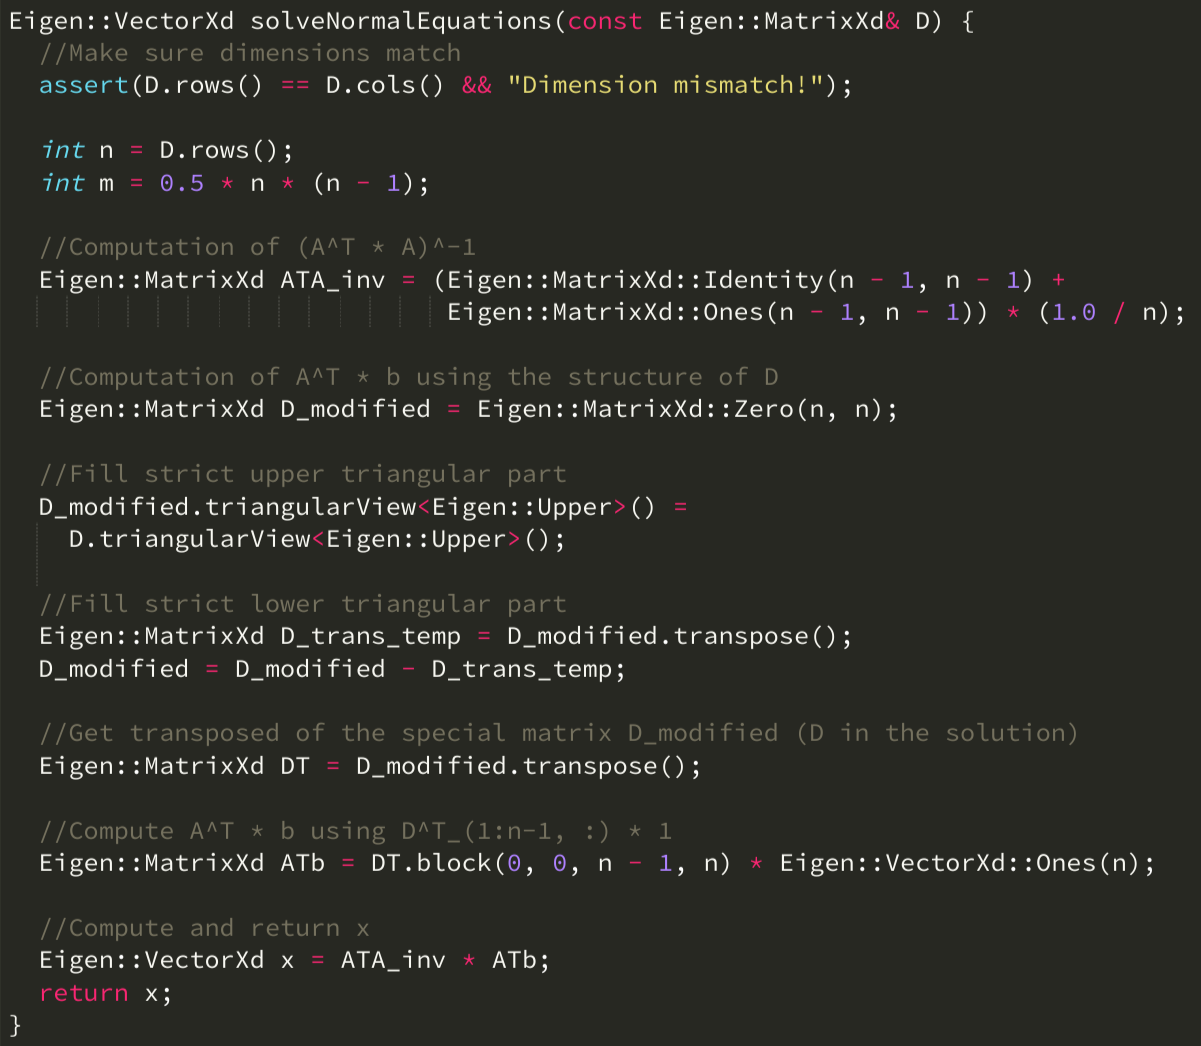
\includegraphics[width=0.9\linewidth]{3-10,e.png}
\end{figure}

\subsection*{3-10.f}
We are tasked with writing a function that calls both solvers we implemented and compares the results and returns \verb|true| if they agree and \verb|false| if they do not. We need to keep in mind that we cannot just compare the result but rather for results $\mathbf{x}_{1}$ and $\mathbf{x}_{2}$ we would choose some error tolerance $\tau$ and check if
\begin{equation*}
    \left\lVert \mathbf{x}_{1} - \mathbf{x}_{2} \right\rVert_{2} < \tau \cdot \left\lVert \mathbf{x}_{\text{better}}\right\rVert_{2}
\end{equation*}
where $x_{\text{better}}$ is the result we expect to the more accurate one, which here we choose the first implantation as it is slower but also uses implementations that are tested and confirmed to be stable built-ins from the Eigen library. This leads to the following code.

\begin{figure}[!hbt]
    \centering
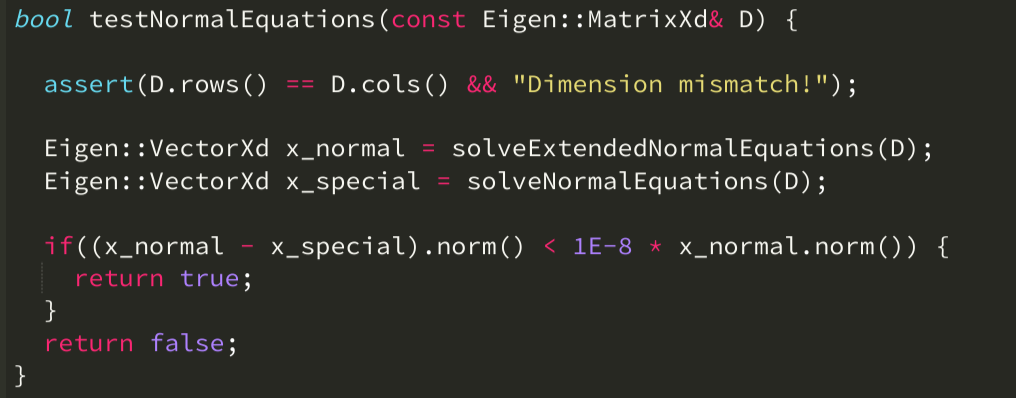
\includegraphics[width=0.9\linewidth]{3-10.f.png}
\end{figure}
\subsection*{3.10.f}
We are tasked with determining the asymptotic complexity of our implementation of \verb|solveNormalEquations()|. Let us go through the code line by line. The computation of $m$ does three elementary operations and is hence in $\mathcal{O}\left(1\right)$, then the computation of \verb|ATA_inv| adds to matrices and then divides every entry by $n$, havin $\mathcal{O}\left(n^{2}\right)$ entries, this means that it takes $\mathcal{O}\left(n^{2}\right)$ operations to do this. We then initialize \verb|D_modified| and set entries on the strict upper and strict lower diagonal which all can be performed in $\mathcal{O}\left(n^{2}\right)$, transposing does not add to the cost (even though it would not surpass $\mathcal{O}\left(n\right)$) as it only changes the interpretation of the matrix, rather than swapping entries in memory, we then multiply the block \verb|DT.block(0, 0, n-1, n)| with the vector $\mathbf{1}$ which takes $\mathcal{O}\left(n^{2}\right)$ as well. Finally we compute one more matrix-vector product ($\mathbf{A}^{\mathsf{T}}\mathbf{b}$ is a vector) which also can be done in $\mathcal{O}\left(n^{2}\right)$. Overall we hence get $\mathcal{O}\left(n^{2}\right)$.


\end{document}
